% !TEX root = ../memoria.tex

\chapter{Materiales, datos y entorno de trabajo}
\label{cap:capitulo4}

En este capítulo se describen los materiales utilizados para el desarrollo del proyecto y la forma en la que se organizaron los datos de partida. También se presenta el entorno físico y software empleado, así como las principales librerías utilizadas durante el procesamiento, entrenamiento y análisis de los resultados.


\section{Protocolo experimental y estímulos auditivos}

Las señales utilizadas en este trabajo fueron registradas en la Facultad de Medicina de la Universidad Complutense de Madrid, en un entorno preparado para la adquisición de señales fisiológicas. Las sesiones se realizaron en una sala controlada, sin iluminación y acondicionada para reducir tanto el ruido acústico externo como posibles interferencias electromagnéticas. Estas condiciones son importantes en registros de \ac{EEG}, ya que la señal tiene una amplitud muy baja y puede verse afectada por movimientos, distracciones o ruido procedente del entorno.

Cada sesión de registro tuvo una duración aproximada de hora y media. Durante la grabación, el participante permanecía en la sala mientras se le presentaban distintos estímulos auditivos diseñados para inducir estados emocionales concretos. Para ello se utilizaron frases sin significado léxico relevante, de forma que la emoción no dependiera tanto del contenido semántico de la frase, sino de la prosodia\footnote{\url{https://es.wikipedia.org/wiki/Prosodia_(ling\%C3\%BC\%C3\%ADstica)}}, es decir, de elementos como la entonación, el ritmo, la intensidad o la forma de pronunciarla.

Los estímulos auditivos se asociaban a las condiciones emocionales consideradas: alegría, tristeza y estado neutro. La elección de este tipo de estímulos permite centrar la respuesta emocional en la forma en la que se escucha la frase, evitando en parte que el significado de las palabras condicione la interpretación del sujeto. De esta manera, las grabaciones obtenidas contienen segmentos de \ac{EEG} relacionados con cada una de las condiciones emocionales que posteriormente se emplean en el proceso de clasificación.

Para la adquisición se utilizó un sistema de \ac{EEG} con un gorro de electrodos humedecidos, lo que mejora el contacto entre los sensores y el cuero cabelludo. Antes de comenzar la grabación era necesario colocar correctamente el gorro, revisar el contacto de los electrodos y preparar al participante para reducir movimientos innecesarios durante la sesión.

\begin{figure}[H]
    \centering
    \subfigure[Sala de grabación utilizada para la adquisición de las señales.]{
        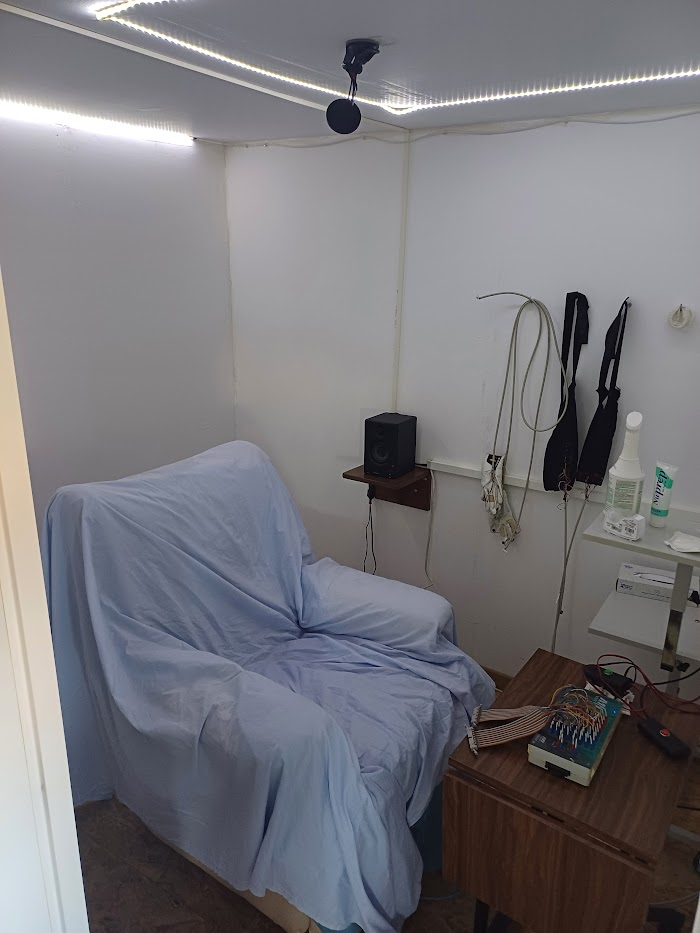
\includegraphics[width=0.45\textwidth]{figs/habitacion_grabacion.png}
        \label{fig:habitacion_grabacion}
    }
    \hfill
    \subfigure[Sistema EEG con gorro de electrodos humedecidos.]{
        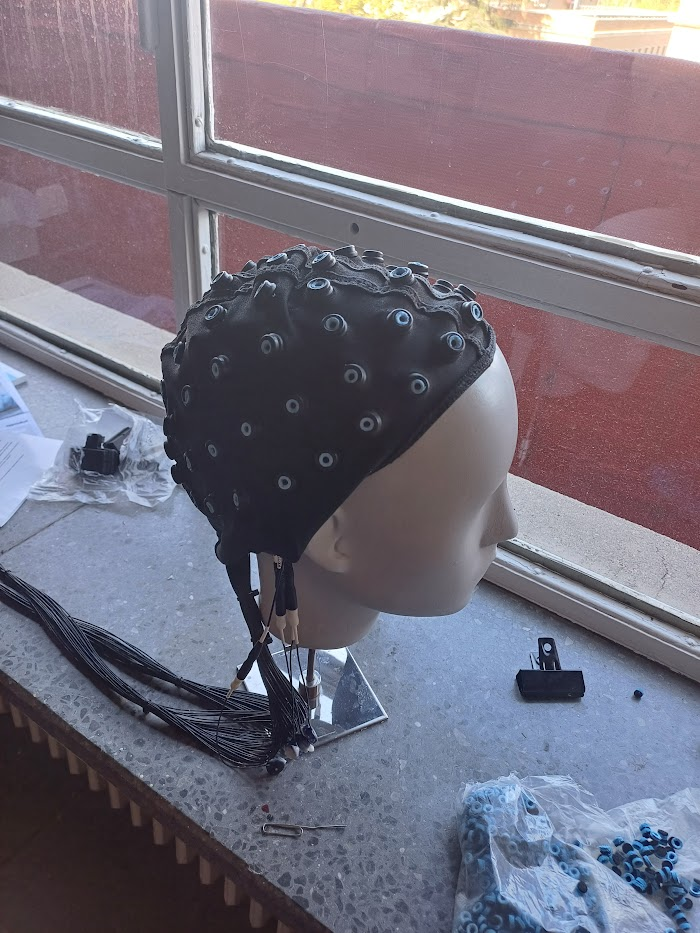
\includegraphics[width=0.45\textwidth]{figs/casco_eeg.png}
        \label{fig:casco_eeg}
    }
    \caption{Entorno y material utilizados durante el registro de las señales EEG.}
    \label{fig:entorno_registro_eeg}
\end{figure}

\section{Descripción general de los datos}

El conjunto de datos utilizado está formado por registros de \ac{EEG} almacenados en el formato \ac{EDF}\footnote{\url{https://www.edfplus.info/specs/edf.html}}. En total se dispone de 72 archivos, correspondientes a 24 participantes y tres condiciones emocionales por participante: alegría, tristeza y estado neutro. Para cada sujeto existe un registro asociado a cada una de estas condiciones, por lo que el conjunto inicial se encuentra equilibrado a nivel de archivos.

Los participantes aparecen identificados mediante códigos anónimos, evitando incluir información personal en los nombres de archivo. Cada archivo sigue una nomenclatura que permite reconocer el sujeto, el número de registro y la condición emocional, por ejemplo \texttt{211-000531-01\_JOY.edf}. En este caso, \texttt{211-000531} identifica al sujeto, \texttt{01} al registro concreto y \texttt{JOY} a la condición emocional.

Cada archivo en formato \ac{EDF} contiene las señales registradas durante una condición experimental concreta. Las cabeceras de los archivos incluyen 66 señales: 64 canales de registro y dos canales auxiliares, \texttt{STIM} y \texttt{SYNC}, utilizados para almacenar información de sincronización y eventos. Los datos descritos en esta sección corresponden al material original de partida, antes de aplicar las etapas de filtrado, segmentación, limpieza o extracción de características.

\section{Organización de los datos en bruto}

\section{Organización del repositorio}

\section{Entorno físico y software de trabajo}

\section{Librerías y dependencias principales}
